\documentclass{standalone}
\usepackage[utf8]{inputenc}
\usepackage{tikz}

\begin{document}
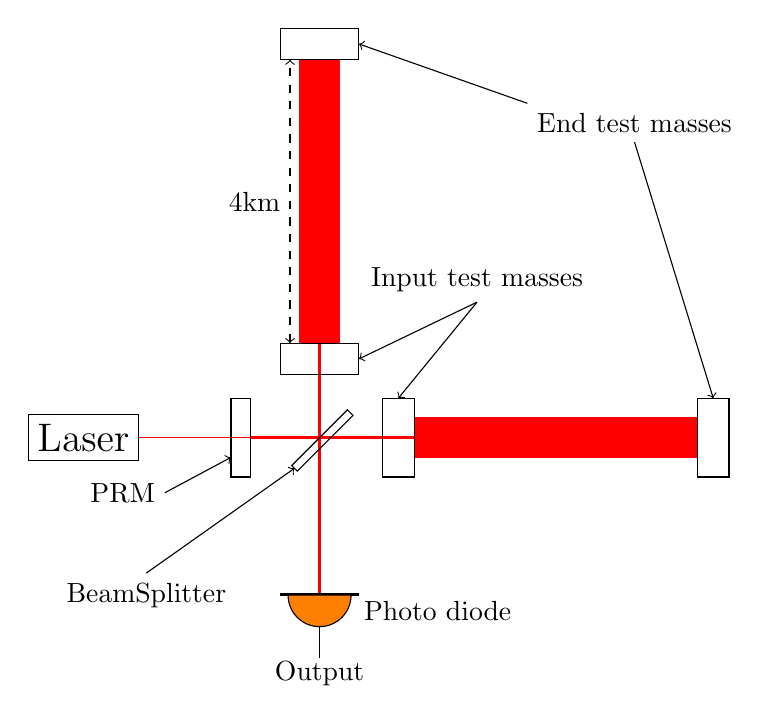
\begin{tikzpicture}
\pgfmathsetmacro{\bsl}{1} % Beam splitter length
\pgfmathsetmacro{\bsw}{0.1} % Beam splitter width
\pgfmathsetmacro{\mw}{1} % Mirror size
\pgfmathsetmacro{\prmw}{0.25} % PRM width
\pgfmathsetmacro{\tmw}{0.4} % Test mass width
\pgfmathsetmacro{\innersep}{1}
\pgfmathsetmacro{\BSx}{\bsw / (2 * sqrt(2))}
\pgfmathsetmacro{\BSy}{-\bsw / (2 * sqrt(2))}

% Coordinates
\coordinate (O) at (0, 0);

% Laser
\node[draw, rectangle] (laser) at ({-3 * \innersep}, 0) {\Large Laser};

% Beams
\draw[red] (laser.east) -- ({-\innersep + \prmw / 2}, 0);
\draw[red, very thick] ({-\innersep + \prmw / 2}, 0) -- (O);
\draw[red, very thick] (O) -- (0, {\innersep + \tmw / 2});
\draw[red, fill=red] ({0 - \mw / 4}, {\innersep + \tmw / 2}) rectangle ({0 + \mw / 4}, {5 * \innersep - \tmw / 2});
\draw[red, very thick] (O) -- ({\innersep + \tmw / 2}, 0);
\draw[red, fill=red] ({\innersep + \tmw / 2}, {0 - \mw / 4}) rectangle ({5 * \innersep - \tmw / 2}, {0 + \mw / 4});
\draw[red, very thick] (O) -- (0, {-2 * \innersep});

% Beamsplitter
\draw[rotate around={-45:(\BSx, \BSy)}] ({\BSx-\bsw/2}, {\BSy-\bsl/2}) rectangle ({\BSx+\bsw/2}, {\BSy+\bsl/2});

% PRM
\draw ({-\innersep - \prmw / 2}, {-\mw / 2}) rectangle ({-\innersep + \prmw / 2}, {\mw / 2});

% North arm
% First mass
\draw ({0 - \mw / 2}, {\innersep - \tmw / 2}) rectangle ({0 + \mw / 2}, {\innersep + \tmw / 2});
%End mass
\draw ({0 - \mw / 2}, {5 * \innersep - \tmw / 2}) rectangle ({0 + \mw / 2}, {5 * \innersep + \tmw / 2});

% East arm
% First mass
\draw ({\innersep - \tmw / 2}, {0 - \mw / 2}) rectangle ({\innersep + \tmw / 2}, {0 + \mw / 2});
%End mass
\draw ({5 * \innersep - \tmw / 2}, {0 - \mw / 2}) rectangle ({5 * \innersep + \tmw / 2}, {0 + \mw / 2});

% PD
\pgfmathsetmacro{\pdw}{0.8}
\draw[black, fill=black] ({-\mw / 2}, {-2 * \innersep + 0.02}) rectangle ({\mw / 2}, {-2 * \innersep});
\draw (0, {-2 * \innersep - \pdw / 2}) -- (0, {-2 * \innersep - \pdw});
\draw[fill=orange] ({\pdw / 2}, {-2*\innersep}) -- ({-\pdw / 2}, {-2*\innersep}) arc(180:360:{\pdw/2}) -- cycle;

% Annotations
\draw[<->, dashed] ({-3 * \mw / 8}, {\innersep + \tmw / 2}) -- node[left] {4km} ({-3 * \mw / 8}, {5 * \innersep - \tmw / 2});
\node at (0, {-2 * \innersep - \pdw - 0.2}) {Output};
\node at (1.5, {-2 * \innersep - \pdw / 4}) {Photo diode};
\node (prmnode) at ({-2.5 * \innersep}, -0.7) {PRM};
\draw[->] (prmnode.east) -- ({-\innersep - \prmw / 2}, {-\mw / 4});
\node (bsnode) at ({-2.2 * \innersep}, -2) {Beam\\Splitter};
\draw[->] (bsnode.north) -- ({\BSx - (1 / sqrt(2) * \bsl / 2)}, {\BSy - (1 / sqrt(2) * \bsl / 2)});
\node (testmassnode) at ({4*\innersep}, {4*\innersep}) {End test masses};
\draw[->] (testmassnode.north west) -- ({0 + \mw / 2}, {5 * \innersep});
\draw[->] (testmassnode.south) -- ({5 * \innersep}, {0 + \mw / 2});
\node (itmnode) at ({2*\innersep}, {2*\innersep}) {Input test masses};
\draw[->] (itmnode.south) -- ({\mw / 2}, \innersep);
\draw[->] (itmnode.south) -- (\innersep, {\mw / 2});
\end{tikzpicture}
\end{document}